
%
%  $Description: Author guidelines and sample document in LaTeX 2.09$
%
%  $Author: ienne $
%  $Date: 1995/09/15 15:20:59 $
%  $Revision: 1.4 $
%

\documentclass[10pt,twocolumn]{article}
\usepackage{latex8}
\usepackage{times}
\usepackage{graphicx}

%\documentstyle[times,art10,twocolumn,latex8]{article}

%-------------------------------------------------------------------------
% take the % away on next line to produce the final camera-ready version
\pagestyle{empty}

%-------------------------------------------------------------------------
\begin{document}

\title{From Sketching Android Application GUIs to Generating Example Code}

\author{Will Hollingsworth, Steven Walker\\
College of William \& Mary\\ Department of Computer Science
}

\maketitle
\thispagestyle{empty}

\begin{abstract}
   Abstract filler.
\end{abstract}



%-------------------------------------------------------------------------
\Section{Introduction}

Introduction filler.

%-------------------------------------------------------------------------


\begin{figure}[htb]
\centerline{
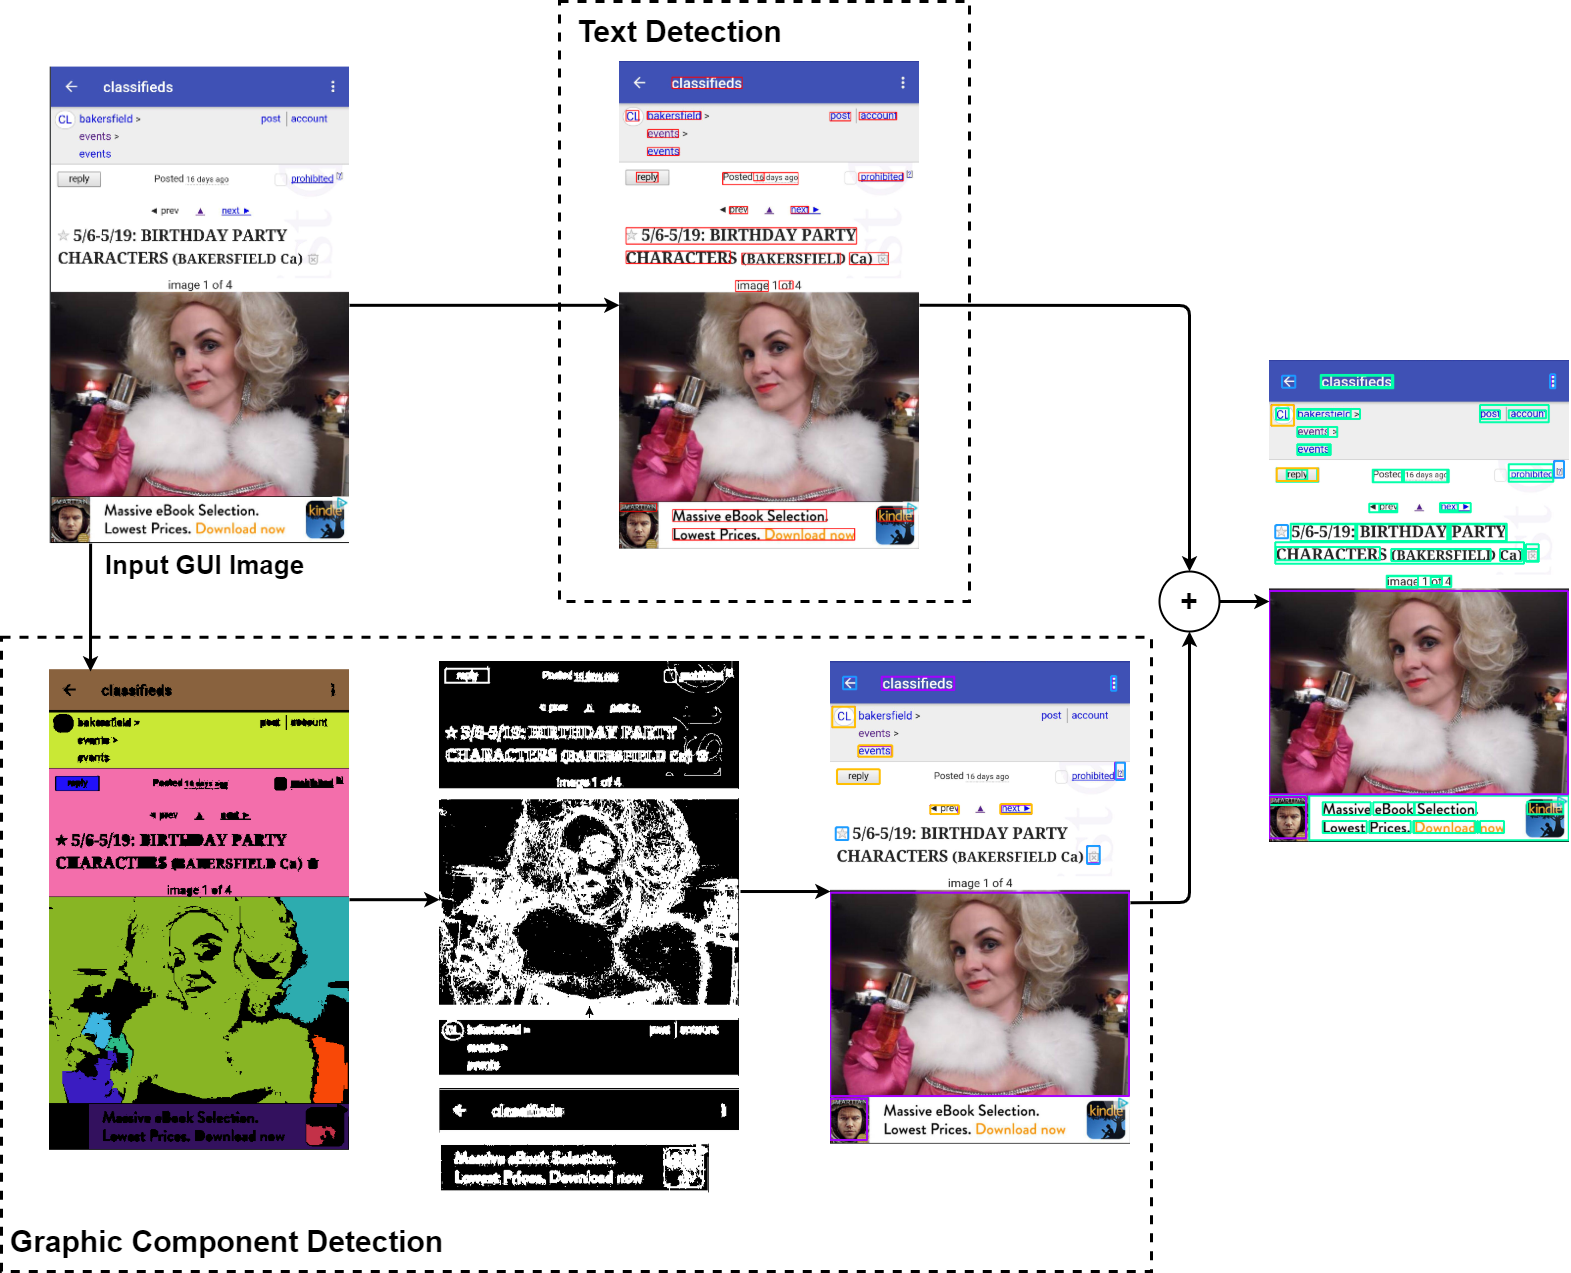
\includegraphics[width=1.0\columnwidth]{approach.png}}
\caption{Overview of our approach, highlighting each of the individual processing steps.}
\label{fig:approach}
\end{figure}

\Section{Approach}

We begin with a high level description of our approach and then will address
each individual step in more detail. Our approach follows a six step pattern
that is based off the REMAUI \cite{remaui} approach, as seen in Figure \ref{fig:approach}. First, we take a GUI mockup that can either be computer generated or hand drawn and pass that into an OCR algorithm (Step 1). The OCR algorithm is used to locate and extract textual elements from the GUI. We use heuristics (explained in Step 1) to eliminate some of the false positives from the OCR algorithm.

The same GUI mockup is also passed into a computer vision system to identify non-textual GUI components in the mockup such as images contained in ImageViews, buttons, and more (Step 2). Computer vision techniques allow us to identify edges and boundaries to all of the GUI components.

The next step is to combine the information gained by using OCR and computer vision (Step 3). Additional heuristics (explained in Step 3) are used by matching the computer vision bounding boxes with the OCR inferred text lines. The goal is to further reduce the OCR false positives.

We then identify lists (Step 4) and use this information to build the GUI in terms of the Android layouts, source code declarations, strings, and images (Step 5). Once these assets are generated, they are used in our source code search engine to locate code examples from similar GUIs (Step 6).

\SubSection{Step 1: Optical Character Recognition}
The image of the GUI mockup is imported into the OCR algorithm. In our implementation, we used Tesseract, an open-source OCR system. Tesseract is used to detect words that are present in the GUI mockup. Due to high false positive rate, a list of heuristics are used to eliminate candidates that aren’t actually words.

Our heuristics eliminate words based on the bounding boxes and contents of the words. They should be non-zero in size, should not have an extreme length:height ratio, should not extend off screen, should contain letters, and should meet an expected size based off the font and font size.

\SubSection{Step 2: Computer Vision}
The second step involves feeding the same GUI mockup into a computer vision system to detect the GUI components. The goal is to identify all GUI components and to identify a view hierarchy. We use OpenCV, an open-source computer vision platform.

The process of identifying view elements starts with running Canny’s algorithm for edge detection. Next to merge close elements, such as characters in the same word, the edges are dilated. Next the contours are identified. Each contour becomes it’s own atomic element. Lastly, a bounding box for each contour is computed.

\SubSection{Step 3: Merging}
After obtaining the computer vision and OCR results, we heuristically throw away
detected ``words'' that conflict with bounding boxes determined by computer
vision algorithms.  For instance, the OCR algorithms occasionally pick up false
positives in the form of images;  since these elements will also be picked up by
the computer vision results, the bounding boses will overlap, and we can safely
remove them from the OCR results.

Furthermore, we combine the results from OCR identifying words and lines and
merge them into text blocks.  This process takes into consideration the distance
between two words; although such words would be recognized as a single line by
the OCR algorithms, the text boxes we generate would separate these.

Using additional heuristics, we eliminate some of the false positives generated
by the OCR algorithms.  First, words detected by OCR should not overlap
significantly with two vision boxes that do not overlap each other.  Words
should not contain single vision boxes whose sizes are significantly smaller
than the word.  The words should contain only vision boxes which are not leaves
in the vision box tree.  Vision boxes that do not overlap should correspond to
only a single word.  We throw away any words such that there are multiple words
with the same text and formatting, and recieved a low confidence from the OCR
algorithm.

\SubSection{Step 4: Compacting View Hierarchy}
The view heirarchy generated in in the previous step may contain redundant
information.  For instance, it may add a layout around every view.  Since this
is not necessary, it is necesary to prune the view heirarchy such that it only
contains the nessecary nodes.  To accopmlish this, we consider each node in the
tree, and check whether it has identical subtrees.

Note that the subtrees are considered identical only if the XML elements are the
same -- the actual content may very.  That is, each subtree being composed only
of a text view is sufficient; the text contained does not need to be the same.
After finding these identical subtrees, we collapse them into a single element.
To continue to text view example, we would collapse the several text views into
a single one, concatenating the text in the original views.

\SubSection{Step 5: Export}
At this stage, we export all results as an Android project.  This includes a
skeleton of the application with a complete GUI element heirarchy.  Android
resource files are generated as well, including the XML files used for strings,
application styling, and application layout.  We care to ensure that resources
are not duplicated.

\SubSection{Step 6: Code Search}
Finally, we compare the generated skeleton code to other applications in a
database by computing their similarity as described in \cite{clan}.  We then
present screenshots of the various application activities for both the generated
skeleton code and the other applications.  This allows the developer to select
possible alternative designs.

%-------------------------------------------------------------------------
\Section{Research Questions}

We aim to answer the folowing research questions:

\begin{enumerate}

\item \textbf{RQ$_1:$}  \textit{Is our system able to effectively capture salient features of mobile app sketches?} Our system should be able to identify key features of Android applications including, but not limited to text, images, lists, and buttons. The application skeleton code our system creates when ran on an Android device should be similar visualy and have a similar view heirarchy as the provided sketch.

\item \textbf{RQ$_2:$} \textit{Are the returned application examples from the code search similar in functionality to the provided sketches?} The example code returned by the code search should have a similar view heirarchy and share a large subset of GUI components.

\end{enumerate}

\Section{Design of Experiments}
To answer our research questions, we implement our approach in \textsc{Reach}, a
freely availble Android tool.

\SubSection{Application Generation Analysis}

To answer \textbf{RQ$_1$}, we borrow an evaluation metric from \textsc{Remaui},
\cite{remaui} noting that each pixel in our generated application should be
contained by the same view as the input sketch.  For instance, if the sketch
contains an image view, then the same pixels it contains should be in an image
view in the generated application.

We formalize this heuristic by defining the \textit{precision} and
\textit{recall} of the generated application.  The recall quantifies how many
pixels contained by a specific type of view in the application is contained by
the same type of view in the sketch.  Precision quantifies how many pixels in
the sketch were correctly classified by \textsc{Reach} and placed in the same
type of view.

We express these mathematically.  For a set of pixels $i$ contained by an image
view in the sketch, and set $i^\prime$ in the generated application, we define
the precision $p_i$ and recall $r_i$ as follows:

\begin{equation}
  p_i = \frac{\left|i \cap i^\prime\right|}{\left|i^\prime\right|}
\end{equation}
\begin{equation}
  r_i = \frac{\left|i \cap i^\prime\right|}{\left|i\right|}
\end{equation}


\SubSection{Code Search Analysis}

The goal of the code search is to return application examples that contain a similar view heirachy and use similar GUI components. The main concern of the code search is with application functionality and not with visual presentation. To compare the similarity of functionality, we do not take into account the visual representation of the matched code such as GUI component size of position on screen. Instead we use some similarity metrics about the view heirarchy and the GUI components contained within it.

The similarity metrics used will cover a range of features the matched application should have in common with the generated application. First, the application should use all of the GUI components (ImageView, TextView, Button, etc) that the generated code uses. Ideally the matched application should have as small of a superset as possible of the GUI components used in in the generated code, but having extra GUI components used is favorable compared to missing GUI components. The percentage of GUI components used in the matched application is our first metric.

In order for the matched application to have similar functionality, the number of GUI components should be almost identical. Our second similarity metric is the ratio for total number of GUI elements used between the matched application and the generated application. This can be broken down further for each GUI component individually and then aggregated by taking the average of the ratios.

There are other similarity metrics which could be used on each GUI component with it's position in the view heirarchy. Some metrics would be the number of siblings, the types of the siblings, number of children, type of the parent view, and depth. Using these pose some challenges due to view containers where sometimes single views may be wrapped in view containers. A solution would be to first remove all view containers which contain only one child view. This would allow for a more direct comparison between the two applications. We leave these additional metrics as future work.
%-------------------------------------------------------------------------
\Section{Results}

Results to be placed here.


%-------------------------------------------------------------------------
\Section{Threats to Validity}

Threats to validity filler.

%-------------------------------------------------------------------------
\Section{Related Work}
\SubSection{Reverse Engineering GUIs}
Most closely related to our work is REMAUI \cite{remaui} which reverse engineers
Android user interfaces, but is currently only available to the public as a web
application.  In contrast, our work is completely open source, and users will
able to make use of our implementation offline.  Our goals also differ
significantly from those of REMAUI.  Rather than using a screenshot as input,
our intention is to allow designers to prototype application GUIs on pen and
paper (as this is generally their preference \cite{}).

Also, although REMAUI successfully generates a runnable Android application with
a complete view hierarchy, it does not implement any functionality.  For
instance, a button appearning in the input screenshot will have a counterpart in
the generated application, that button will not have any \verb\onClick()\ method
associated with it.  Our goal is to provide such functionality by way of code
search.  Specfically, we aim to leverage source code from existing applications
with GUIs similar to the provided prototypes.  In this way, we hope to provide
developers with options regarding the appearance of the generated, working application.

MobiDev \cite{mobidev} also reverse engineers mobile app GUIs, and also provides 
a means of creating and sharing applications on smart devices themselves.  
Developers can create a GUI using a graphical editor, or by creating a sketch 
made using a visual UI description language, where specific structures can be 
drawn to correspond to different widget types.  A photo of the sketch can be 
taken with the device's camera and polished with the graphical editor.  Reach is 
similar in that it accepts as input prototype sketches, but additional 
development is intended to be done in a more traditional environment.  MobiDev 
also does not perform a code search for similar apps.

JavaSketchIt \cite{sketchit} defines a more rigoruous visual grammar which 
allows for interactive digital editing of GUI prototypes, using fuzzy logic to 
remove some of the ambiguity in human drawings.  The described grammar is 
reasonably intuitive and can be used to create an application writing in Java.  
Our approach differs in that we aim to allow designers to develop prototypes on 
paper.  Also, since Android GUIs are defined primarly though XML configuration 
files, the output of our system is significantly different.

Accessibility APIs provide low level information regarding GUI elements on
screen.  Chang et al \cite{accessibility} developed a framework combining this
metadata with pixel level data.  This framework provides the basis for high
level operations on the GUI itself, such as copying and pasting widgets.

Silva et al. \cite{staticAndDynamic} reverse engineer web applications using a
combination of static and dynamic analysis.  In their method, whenever the user
interacts with a widget in a running application, a static analysis is performed
on the event handler associated with that widget, thus providing the benefits of
both methods. Our work relies solely on static analysis and does not require an
existing application, hand drawn designs work as well.

\SubSection{Code Searching}
Our method searches for Android application source code for similar GUIs.
Previous work for searching for similar applications include CLAN \cite{clan}
and Exemplar \cite{exemplar}. CLAN \cite{clan} computes a similarity index of
two Java applications based upon the API calls used.  APIs are weighted based
upon how commonly they appear in applications.  This is done with the
observation that similar applications are likely to use similar APIs.  Our
approach is closet to CLAN in that we determine the similarity between
applications, but we provide developers of screenshots of the actual Android
activities.

Exemplar \cite{exemplar} begins with a high level description of an application
that a developer wishes to build, and searches API documentation for matching
keywords.  The developer is presented with a list of applications using the
associated API calls.

Portfolio \cite{portfolio, portfolioMillions} visualizes a call graph for API
calls relevant to a search query.  The font size of the method names is adjusted
based upon the method's overall relevance to the search query.  Although we
provide the developer with a visualization, this will be of actual Android
activities rather than simply method calls.

%-------------------------------------------------------------------------
\Section{Conclusion}

Conclusion filler.

%-------------------------------------------------------------------------
%\nocite{ex1,ex2}
\nocite{*}
\bibliographystyle{latex8}
\bibliography{latex8}

\end{document}

